\graphicspath{{figures/AcceptanceTest/}}

\section{Inverted Pendulum Acceptance Tests}\label{sec:InvPendAccTest}

In this section the tests to check whether the controllers designed for the inverted pendulum fit the requirements or not. As said in \autoref{sec:TestDesc} the first acceptance test will not be documented as it more an implementation requirement than a test.

\subsection{Acceptance Test 2.}

The goal of this test is to see if the inverted pendulum's stick and arm stay within the limits set in Requirement 2 and 3 describe in \autoref{sec:InvPendReq}. \autoref{fig:AccTest2} plots the angles of the arm and the stick over a period of \SI{30}{\second} the maximum and the minimum angles are put in evidence so that it is easy to compare them with the requirements.

\begin{figure}[htbp]
	\centering
	\begin{subfigure}{0.45\textwidth}
		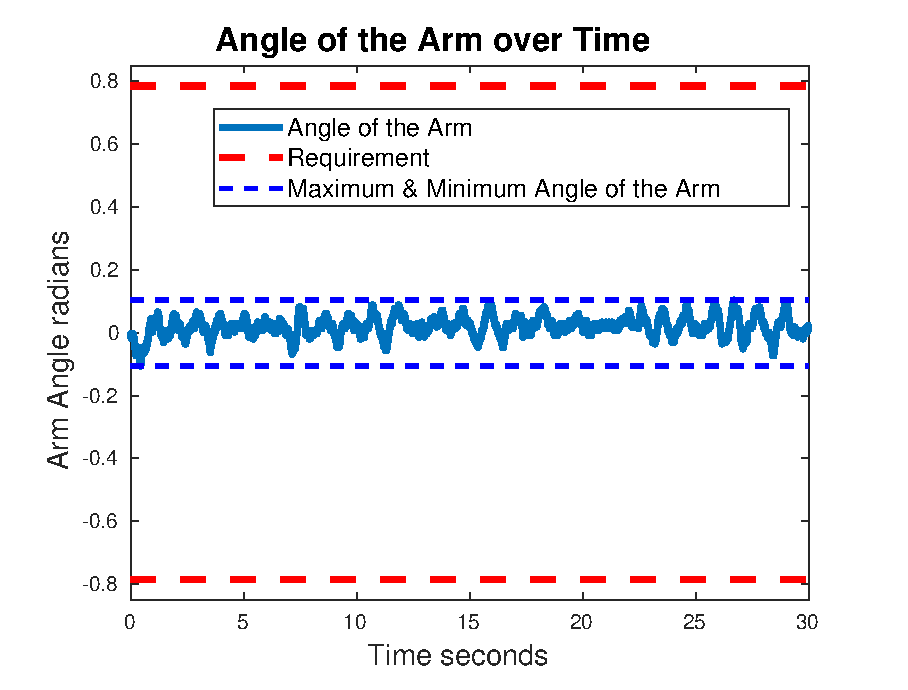
\includegraphics[width=\textwidth]{AngleArmplot}
		\caption{Plot of the angle of the arm.}
	\end{subfigure}
	\begin{subfigure}{0.45\textwidth}
		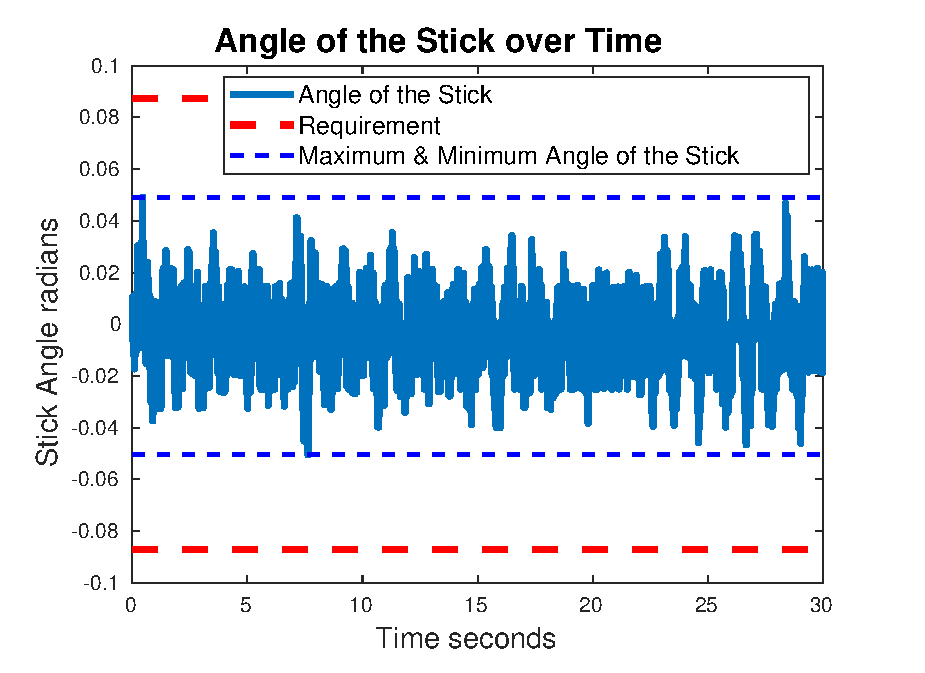
\includegraphics[width=\textwidth]{AngleStickplot}
		\caption{Plot of the angle of the arm.}
	\end{subfigure}
	\caption{Plot of the angle over time with the limits set by the requirement.}
	\label{fig:AccTest2}
\end{figure}